\documentclass[a4paper,11pt]{article}

\usepackage{graphicx}
\usepackage{natbib}
\usepackage[utf8]{inputenc}
\usepackage{tabularx}
\usepackage{hyperref}
\usepackage{color}
\usepackage{float}
\usepackage[usenames,dvipsnames,svgnames,table]{xcolor}
% \usepackage{mathptmx} % Times New Roman

\setlength{\topmargin}{-0.4mm} % (1in=25.4mm)-0.4mm=25mm
\setlength{\textheight}{243.119mm} % 297mm-40mm-10mm-(11pt=3.881mm)=
\setlength{\oddsidemargin}{-0.4mm} % (1in=25.4mm)-0.4mm=25mm
\setlength{\textwidth}{160mm} % 210mm-50mm=160mm
\setlength{\headheight}{0mm}
\setlength{\headsep}{0mm}
\setlength{\footskip}{15mm}

\providecommand*{\note}[1]{\small \textcolor{RoyalBlue}{\begin{minipage}{\textwidth}{#1}\end{minipage}}}

% --------------------------------------------------------------

\providecommand*{\ShortTitle}{WaveMeIn}
\providecommand*{\FullTitle}{WaveMeIn: Authentication via Brain Waves}

% --------------------------------------------------------------

\title{\textbf{\sffamily\Huge \ShortTitle}\\ 
{\textbf{\sffamily\Large \FullTitle}}
\vspace{1cm}}

\author{
{\em 188.407: Management von Software Projekten} \vspace{1cm} \\
Group: 10\bigskip \\
Belk Stefan \\ {\small 0750926, 937, \href{mailto:belk.stefan@gmail.com}{belk.stefan@gmail.com}}\\
Petz Thomas \\ {\small 0601280, 937, \href{mailto:e0601280@student.tuwien.ac.at}{e0601280@student.tuwien.ac.at}}\\
Causevic Alma \\ {\small 0847805, 534, \href{mailto:alma.causevic@hotmail.com}{alma.causevic@hotmail.com}}\\ 
Causevic Amra  \\ {\small 0649241, 534, \href{mailto:amra.causevic@hotmail.com}{amra.causevic@hotmail.com}}\\ 
Seebacher David \\ {\small 0327243, 534, \href{mailto:david.seebacher@student.tuwien.ac.at}{david.seebacher@student.tuwien.ac.at}}\\
\vspace{4cm}
}

\begin{document}

\begin{titlepage}
\maketitle

\end{titlepage}

% --------------------------------------------------------------

\thispagestyle{empty}
\tableofcontents
\pagebreak

\setcounter{page}{1}


% --------------------------------------------------------------

\note{
\textbf{Formal constraints}
\begin{itemize}
\item	  Font: Times New Roman oder Computer Modern (\LaTeX default)
\item    Fontsize: 11pt
\item     Single line spacing
\item     Margins: 2.5cm side and top/bottom
\item     \fbox{Language: ENGLISH}
\item    The proposal template should be filled incrementally. I.e., at the end there should be a full project proposal in a single PDF file.
\end{itemize}
\textbf{Available templates}
\begin{itemize}
\item     Proposal (mswp-proposal.tex)
\item     Costs (costs.xls, costs.ods)
\end{itemize}
\textbf{Supplemental material}
\begin{itemize}
\item     FWF salary scheme (\href{http://www.fwf.ac.at/de/projects/personalkostensaetze.html}{http://www.fwf.ac.at/de/projects/personalkostensaetze.html})
\item     Travel cost regulation (\href{http://www.fwf.ac.at/de/faq/reisegebuehrenvorschrift.html}{http://www.fwf.ac.at/de/faq/reisegebuehrenvorschrift.html})
\item     Ethical issues form (ethical-issues.rtf)
\end{itemize}
}
\pagebreak

% --------------------------------------------------------------
\section{Synopsis}
\label{sect:synopsis}
\subsection{Project Idea}
WaveMeIn is a research project to create a new type of secure login mechanism. It consists of a small device worn by the user at the ear which authenticates the user based on brain waves.

\subsection{Why do we need it?}
At the time of this proposal the most used ways for authentication are manually typed passwords or biometric authentication methods. However all of the previous methods have some security problems or are simply not user-friendly. Typed passwords are easy to spy out simply by looking at the keyboard of the user or the traces of the fingers on touch displays. In the case of biometric authentication, there are for example face recognition, iris or fingerprint scans. Face recognition software can easily be tricked by face masks or photographs and moreover depends on good light conditions, the quality of the images of the web camera and other factors. Fingerprint and iris scans are the most secure options of the authentication methods mentioned before. However they also have many disadvantages. Iris scans are not practical since the hardware required cannot easily be integrated into small devices and it is not user-friendly to require the user to place his eye very close to the scanner every time he/she wants to unlock a device. Fingerprint sensors are known to fail to recognize the fingerprint correctly quite often and it is also a not very user-friendly authentication method for handicapped people that may not reach the sensor or may not have any fingers at all. 

\subsection{How does it work?}
Brain waves are a secure and user-friendly alternative authentication method. The idea is to create a small device, called Wavy, that can be worn at the ear of the user in the same style as bluetooth headsets are already worn for communication today. The Wavy measures the brain waves near the ear in case a login is required by a client device that is connected via bluetooth. It listens for a brain wave pattern that was previously trained by the user as a password. If the correct pattern was detected by the Wavy it transmits a OK signal back to the client device. 

\subsection{Why should somebody care?}
Nowadays people are forced to type their passwords in public places which is a security risk and also not a very efficient way for authentication. Especially when typing in password on small devices such as mobile phones this authentication method is also very error prone due to the small keyboard interfaces. On the one side people are lazy and do not want to remember and enter long and complicated passwords, but on the other side they are also concerned about the security of their data and their privacy. So the users are in need of a more secure and easier way of authentication.

\subsection{Who are the beneficiaries of the results?}
Basically everybody can benefit from the WaveMeIn project since it is usable in the daily life. Especially for handicapped people it is a new and more easy to use option to log into their devices. Also it grants a higher level of security than existing authentication methods so it is also well suited for environments where higher security is needed, such as access authentication is modern research labs and government or military facilities.

For our product to succeed, we need to invest into research in the area of brain wave detection and analysis. This investment can improve our understanding of this topic. After a commercial success, we have to enhance our product. This means we have to invest further into brain wave research. On the other side, we can make our world more secure. It makes hacking of accounts and password fraud more complicated.

\subsection{Problem classification}
The task of detecting brain waves it tightly connected to the research areas of Neuroscience, Pattern Recognition and Machine Learning. In the field of Neuroscience it touches the areas of not invasive brain computer interfaces and neural oscillation. Since detecting and reliably identifying brain waves at the location near the ears is still technically immature the project can be seen as basic research in this area. The following research questions have to be answered before a prototype can be developed.
\begin{itemize}
	\item Detecting braves at the ears
	\item Recognize brain wave patters
	\item Distinguish correct patterns from random signals
	\item Distinguish brain waves from different users
\end{itemize}
On the other hand if we take the Wavy into account, which should be the resulting product, this project is also an applied research project. It further touches the fields of computer security and privacy.



% --------------------------------------------------------------
\section{Introduction and problem description}
\label{sect:intro}
WaveMeIn is a research project to show the potential of brain waves a new method of electronic authentication via a small wearable device. Its aim is to investigate the usage of rain waves to replace passwords or other authentication methods. Therefore the properties of brain waves regarding uniqueness and reliability have to be explored. The project shall demonstrate via a small prototype that the recognition is possible without large sensors on top of the users head. A requirement for such a method of authentication clearly exists as demonstrated by the following use cases:

\subsection{Current Situation}


\subsection{Use Case 1}{
Assume a user needs to log on to a device (e.g. a notebook) that contains sensitive information in public. Typing in the password is not an option as it can easily be monitored by another person. Fingerprints are also not a good alternative as they can easily be taken from any surface the user touched and be copied onto synthetic materials to deceive the fingerprint reader. Brain waves are (as of current knowledge) unique for each person even if two people are having exactly the same thought. If the intruder does not know the precise brain wave pattern of the user's pass phrase/thought it is impossible to duplicate.}

\subsection{Use Case 2}{
Assume an average user wants to unlock his/her smart phone in a crowded area such as the subway. Nowadays this is done by entering a pin or drawing a pattern on the screen. A person with the intention to steal a users phone just needs to observe its victim while entering the pass code or pattern. Afterwards it is easy to unlock the phone and steal the victims personal data or cause large costs while using it for phone calls and mobile data. Locking the phone via a brain wave authentication mechanism may not prevent the theft but the costs arising from the phone being used afterwards.}

\subsection{Current Authentication Methods}
In theory brain waves will be rank among the most secure authentication methods, probably being the most secure one if the research proves successful. The particular brain wave of a user required to unlock a device can not be easily be obtained other than strapping the user to a chair and forcing him/her to think his/her pass thought. Other authentication methods are password, drawing patterns, fingerprint, iris scan, voice recognition. Passwords and pattern drawing are the least secure ones as the user can be observed while typing or drawing without much effort. Fingerprint, iris scan, voice recognition may require more technical or social effort to obtain, but in the end all of them are features of a person that are always visible for the outside world and therefore copyable with more or less effort.

\subsection{Unresolved Problems and Opportunities}
The unknown factor of this research project is that no research has been done on measuring brain waves at other locations (e.g. the ears) of the body except directly at the users head. Additionally it is unknown if the brain waves of are person are distinctive enough to distinguish a pass thought of a user from other thoughts and if the brain waves of different users while thinking the same thought are distinctive enough.

At the time of writing this proposal there exists no device that is capable of the features mentioned above as well as being small enough to be worn as an accessory. Therefore this is an important area of research with practical future applications.

\subsection{Terms}
\begin{itemize}
	\item 
	\item Brain waves:
	\item
\end{itemize}

% --------------------------------------------------------------
\section{Project goals and deliverables}
\label{sect:goals}
The following sections will provide an overview over the research questions and hardware questions associated with the project.
\subsection{Research questions}
\begin{itemize}
	\item How can be brain waves be detected by the a small device at a single location?
	\item How reliable is the detection of individual brain waves of the same person?
	\item How reliable is unique identification of the brain waves of different persons?
	\item Is it possible to detect brain waves at other body locations than the head?
\end{itemize}

\subsection{Hardware Design}
\begin{itemize}
	\item How can the required hardware be minimized to be small and practical (Wavy Device)?
	\item Are the existing sensors for measuring rain waves good enough for the projects requirements?
\end{itemize}

\subsection{Expected Results}
\begin{itemize}
	\item Successful research on the identification of brain waves.
	\item Algorithms to reliably identify brain wave patterns.
	\item Creation of a small prototype device capable of reading brain waves.
\end{itemize}

At the end of the project it should be clear if:
\begin{itemize}
	\item The detection of brain waves is possible at different locations of the body.
	\item The same thought produces a repeatable and reliable brainwave pattern. (Reliability)
	\item Different people have different patterns when thinking the same thought. (Uniqueness)
	\item Brain waves can be used as authentication method.
	\item The necessary can e integrated into a small device.
\end{itemize}

\subsection{Non-Goals}
\begin{itemize}
	\item No mind reading device
	\item No client software (just the brain wave research, hardware and interface)
	\item No design or usability study (just a prototype that works and is small enough)
	\item No end-user/consumer product (just a prototype)
\end{itemize}

% --------------------------------------------------------------
\section{Scientific relevance and innovative aspects}
\label{sect:relevance}

%\note{
%\begin{itemize}
%\item {\em Length: 1-2 pages}
%\item Why is the project scientifically interesting?
%\item Did others point out that this is an open question?
%\item What are the innovative aspects that make it interesting?
%\item How could the project break new ground scientifically?
%\item To what extent are the objectives ambitious and beyond the state of the art (e.g. novel concepts and approaches or development across disciplines)?
%\end{itemize}
%}
% % % % % % % % % % % % % % % % % % % % % % % % % % % % % % % % % % % % % %
WaveMeIn can be seen as an important step in the development of brain-computer interfaces used on a daily basis. Given the huge possibility, many private corporations as well as research institutes initiated promising projects. To get a quick overview see Section \ref{sect:star}.

\subsection{Simple step into real life}
The use case of brain wave controlled interaction in WaveMeIn is still kept simple, as it is used only to unlock a device and no further commands have to be recognized. On success, following projects can base more sophisticated ways of interaction on results of WaveMeIns research. Even if this project covers a lot of ground work as well, the focus is to create a product usable on a daily basis. Therefore it goes a little further then most other project in this field, as they concentrate on mostly one specific aspect.

\subsection{Brain wave recognition}
In the field of neuroscience the main question will probably be, what kind of brain waves produce recognizable patterns of the same imagination. Another question is, under what circumstances do brain wave scans look similar. Does the pattern change if the context of the person changes, like a noisy environment, strong emotions or the effect of drugs?
The link to pattern matching in computer science would be, how to match the original password-pattern, recorded in a probably neutral state and the input-pattern within a shifted context. This leads to the question, if a brain wave pattern can be normalized without knowledge of the specific context.

\subsection{BCI improvement}
In conjunction with electrical engineering the BCI itself should be revised. The goal is to shrink the scanner to a minimum so it does not disturb while wearing it for many hours in public. There not only size matters but the position of the scanner should be as flexible as possible. That said, a scanner with the proportions of a Bluetooth headset seems appropriate but not feasible at the moment. One task is to raise the level of detail of the scanners and in the same time to suppress undesired noise. It is still unclear what areas of the head are viable to work with an even improved non invasive BCI.

\subsection{Device security}
Since WaveMeIn is not only meant to simplify the unlock mechanism, but to raise the security of the procedure as well, this will be an important task in the area of computer science. The password itself is an interpretation of a specific thought and therefore never conventionally visible as maybe a fingerprint or a typed password. But still, it will be scanned, processed and the interpretation itself or at least a answer will be sent to the device that is waiting to get unlocked. The most vulnerable moment is during transport of the data. The security requirement should be comparable to wireless networks or Bluetooth connections and is therefore a well researched area already.

%* security: since the password in this case, the bw pattern is never shown in public, the transport from the sensor to the computer is the primary attack vector (!?) -> tight protocoll and gadget encryption is a must

%The task of detecting brain waves it tightly connected to the research areas of Neuroscience, Pattern Recognition and Machine Learning. In the field of Neuroscience it touches the areas of not invasive brain computer interfaces and neural oscillation. Since detecting and reliably identifying brain waves at the location near the ears is still technically immature the project can be seen as basic research in this area. The following research questions have to be answered before a prototype can be developed.
% % % % % % % % % % % % % % % % % % % % % % % % % % % % % % % % % % % % % % % % % % %

%http://www.technologyreview.com/news/513861/samsung-demos-a-tablet-controlled-by-your-brain/
%\em{http://www.essp.utdallas.edu/uploads/Main/Publications/WH2013\_Demo\_Paper.pdf}
% --------------------------------------------------------------

\section{State of the art / current knowledge}
\label{sect:star}
\subsection{What results and approaches have already been presented in this or related areas?}
\chapter{1. Berkeley researches replace passwords by measuring brainwaves as a biometric identifier}
\href{http://people.ischool.berkeley.edu/~chuang/pubs/usec13.pdf}
The US Berkeley represents an approach, which turns the brain activity of an user into a biometric identifier. To do this, the Berkeley researchers use a 100 dollar commercial EEG (electroencephalogram), which resembles a Bluetooth headseat with an electrode. This electrode is placed on the users forehead, over the brain's left frontal lobe. The electrode measures the users brainwaves and transmits them via a Bluetooth link to a Device. According to the Berkeley researchers this system has an error rate of below 1 percent.

To ensure that the brain waves of every single person are unique and that they provide enough information to authenticate the user's identity, the Berkley researchers performed tests with participants, which included different kind of tasks. For example, the participants where asked to just sit and focus on breathing in and out, imagine moving their finger up and down and listen for an audio tone. The participants where also asked to focus on a personalized secret, such as singing a song of their choice. During this tasks, the participants where wearing the EEG which measured their brain waves. As result came out, that not only the measured brainwaves of personalized secrets, but also measured brainwaves of simple tasks, like sitting and focusing on breathing, provided a pattern which makes it possible to authenticate an identity.
\begin{figure}[H]
	\centering
    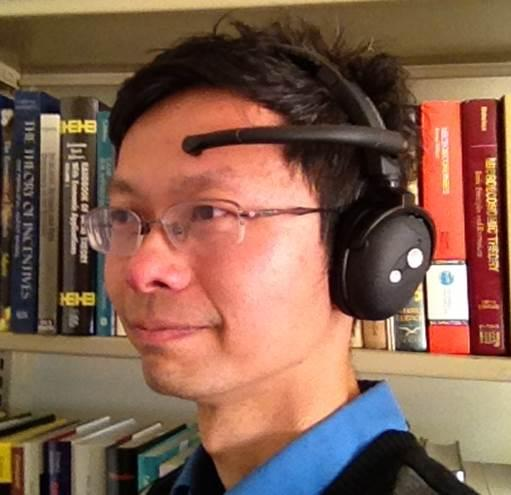
\includegraphics[width=0.5\textwidth]{john_chuang}
    \caption{Professor John Chuang with the Neurosky MindSet brainwave sensor.}
\end{figure}
\chapter{2. Using Brain Waves as New Biometric Feature for Authenticating a Computer User in Real Time}
\href{http://www.cscjournals.org/manuscript/Journals/IJBB/volume7/Issue1/IJBB-211.pdf}
Using brain waves as a biometric Feature for Authenticating was proposed by Kusuma Mohanchandra, Lingaraju G M, Prashanth Kambli \& Vinay in the International Journal of Biometrics and Bioinformat. In this work it has been proved that the brain-wave pattern of every individual is  unique and the signals captured through the  EEG can be used for biometric authentication. This research team used an EEG EPOC headset with 14 channels to measure the brain waves. The collected data, containing the fusion of delta, alpha, theta, beta and gama brain waves, was merged with the aim to create a way to authenticate the user.

There are three basic forms of authentication; something-you-have, something-you-know, and something-you-are.
\begin{itemize}
\item Something-you-have can be objects like a key or passport and people have to be very careful not to loose the object or get it stolen.
\item Something-you-know is based on secret knowledge like passwords or PIN codes and the secret must never be written down, forgotten, or told to others.
\item Something-you-are involves person specific features like fingerprints, voice, face, and gait. Authentication based on such features is called biometric authentication. Brain wave based authentication is a combination of something-you-know and something-you-are when the person involved has to think about something specific, but it can also be just something-you-are when the brain waves are used directly as a biometric.
\end{itemize}
 
The most important part of any authentication system is that true identities (clients) are verified and that false identities (impostors) are rejected. In a password system the password is either right or wrong, but with biometric authentication there is an uncertainty involved because the equipment that  measure the biometric feature rarely provide exactly the same data twice. The reason is that external parameters like finger placement, head rotation, facial hair, location etc are present. The challenge is to overcome these problems in such a way that even two slightly different sets of data can be verified to originate from the same person. There is usually a threshold that decide how different
two different sets of data is allowed to be before they are rejected, and as a consequence there is a chance that some clients are falsely rejected and some impostors are falsely verified.
Biometric authentication therefore introduce two error rates; False Non-Match Rate (FNMR), the rate at which clients are falsely rejected by the system, and False Match Rate (FMR), the rate at which impostors are falsely verified by the system. As such the main problem in this thesis is two compare two or more EEG signals and decide whether they are from the same person or not, and get as low FNMR and FMR as possible.

\chapter{3. Google Glass hack allows brainwave control}


\subsection{Relation to the international scientific work in the field (international status of the research)}
The brain consists of billions of brain cells called neurons. This neurons have to communicate with each other. For this communication the neurons use electricity called brain waves. This communication is producing a lot of brain waves, which can be detected using sensible sensors such as an EEG. The first person, who confirm the existence of brain waves and perform the first tests was Hans Berger. There are five different kinds of brain waves and all of them are directly connected to what a person is thinking, doing and feeling.

\begin{itemize}
 \item Gamma (27 Hz and up)
 \item Beta (12 Hz - 27 Hz)
 \item Alpha (8 Hz - 12 Hz)
 \item Theta (3 Hz - 8 Hz)
 \item Delta (0.2 Hz - 3 Hz)
\end{itemize}

The very beginning of the existence of brain wave based authentication systems dates back to the 1960's when Vogel discovered a connection between a person's EEG signals and his/her genetic code(DNA). It was proved that every person owns unique brainwaves and it possible to identify a person through his brainwaves. Identical twins where shown to have the same EEG patterns in the same situations and even changes related to aging were similar. 


This was also explored by Benedicenti L., Koles’ Z., Mahovsky J., \& Paranjape, R. in the year 2001. This researchers used EEG directly as a biometric and their work showed some promising results on this field.


EEG based person authentication was first proposed by Marcel and Millan in 2007 in “Person authentication using brainwaves (EEG) and maximum a posteriori model adaption”. They proposed the use of  Power Spectral Density as the feature, and a statistical framework based on Gaussian Mixture  Models (GMM) and Maximum A Posteriori Model (MAP) Adaptation on speaker and face  authentication. The potential of their method is shown by simulations using strict train/test protocols and results. 

In 2001 Poulos, Alexandris and Evangelou performed person identification based on spectral information and presented their results in their work: “On the use of EEG features towards oersin identification via neural networks”. To prove the connection between a person's EEG and genetically specific information, this researchers did experiments with the EEG data of healthy individuals. The proposed method has had a success rate of 80 percent to 100 percent showing that the EEG holds genetic information, which can be used for person identification.


Furthermore, a novel two-stage biometric authentication method was proposed by Palaniappan in 2008 (“Two-stage biometric authentication method using thought activity brain waves”). Their results show that the combination of two-stage authentication with EEG features has good potential as a biometric as it is highly resistant to fraud.

\subsection{Description and critical discussion of related scientific work}
The approaches that have been discussed above have succeeded to prove the connection between a person's DNA and her/his brain waves. The approaches clearly show that every single person possesses unique brain waves, which can be used to identify a person. However, a large disadvantage of all of this approaches is that they require the user to wear a big headset with an electrode going across his/her forehead. None of this approaches has succeeded in measuring brain waves from different body parts in order to enable a smaller headset and therefore make it easier for the user to use it in their everyday life.


\note{
\begin{itemize}
\item {\em Length: 2-5 pages}
\item What results and approaches have already been presented in this or related areas?
\item Relation to the international scientific work in the field (international status of the research)
\item Description and critical discussion of related scientific work
\end{itemize}
}

% --------------------------------------------------------------
\section{Method}
\label{sect:method}
\subsection{How should the expected results be achieved?}
In the first place some basic research about brain waves should be done in order to achieve the expected results and build a device for brain wave based authentication. The goal of the projects research part is to clarify the scientific requirements needed for the creation of the prototype. There are two main scientific questions that need to be answered. First, confirm the uniqueness of brain waves or define how specific brain waves of a person can be identified. This is important since we want to assure that the user can be identified as the same one later again. It should be guaranteed that thoughts provide a reliable identification method, therefore the research should give answers how reliably brain waves of a person can be identified. 
Second, besides confirming the uniqueness of a persons brain waves compared to the brain waves of others, another important factor is to confirm that the brain waves of a specific thought of a person are distinguishable from other thoughts of the same person. To prove our assumptions about the uniqueness of brain waves experiments will be conducted on human subjects in the empirical part of this project.  

The research part consists of two phases – a theoretical and an empirical research part. The purpose of the theoretical part is to analyse existing studies and use the results for the project. Already existing studies confirmed the possibility of authentication via brain waves, but so far no study managed to measure brain waves from different head parts than the forehead. The studies showed theoretical approaches to measure brain waves using EEG electrodes placed at the users forehead. The goal of the theoretical research part is to use this approaches and sensor minimising methods in order to define requirements for building a small device, called Wavy. Therefore, the goal to measure brain waves from different head or even body parts is a very important part of the research. The Wavy device should be as small as possible and designed in a way which allows the user to wear it in everyday life. The ears will be the primary focus of this research for measuring brain waves at positions less visible then the forehead. This will enable the Wavy device to be worn like an accessory on or behind the ear. 

In the empirical part there will be some practical tests with human beings, where their brain waves will be measured with an EEG in different situations. The goal of this research part is to confirm the uniqueness of two peoples brain waves, even if they think about the same thing. The approach from UC Berkeley, which John Chuang presented at the 17th International Conference on Financial Cryptography and Data Security, is a good one to use for the project. In this approach the participants were asked to perform seven mental tasks. These were divided into two categories. For the first group of tasks - which was the same for all participants - the subjects were asked to do simple things, for example to focus on their own breathing, imagine moving a finger, or to listen for an audio tone and respond to that by focusing on a dot on a piece of paper. For the second group of tasks - which participants selected and performed individually without letting others know what they were doing - the subjects were asked to select from imagining performing a repetitive motion from their favourite sport, such as swinging a golf club; singing a song of their choice; watch a series of on-screen objects and silently count those that matched a color of their choice; or think of something for 10 seconds. \cite{Adhikari13} These tests will be repeated over several weeks to verify the critical uniqueness of a person's thoughts as mentioned above a prolonged period of time. With such tests the Berkeley researchers managed to ensure that brain waves provide enough information to authenticate the user's identity. This kind of tests will be also done with users in our empirical research part.

\subsection{What methods will be applied?}
The following methods will be used:

\subsubsection{Theoretical study}
The goal of the theoretical study is to gather information from existing studies on this field. Several different studies already investigated the possibility of using brain waves as access method. Their findings will be used as a start point for our research. Researchers in the field of neuroscience and computer science will be needed for this task which will be part of the first work packages at the beginning of the project.

\subsubsection{Experiments}
This part consists of performing practical tests with participants. During these tests the users will wear an EEG device and will be asked to think of some simple things as well as thinking of some personal memories or for example their favourite song. 
The experiments will define whether brain waves of every single person are unique and how reliable they can be measured from different body parts. The participants will have to be selected as heterogeneous group so that the experiments can be performed on people with different characteristics such as male/female, adult/children, etc. Neuroscience and computer science are the required fields of expertise for this part. The results of the experiments will also determine which sensors are best suited for the future prototype. The human brain produces a wide range of different brain waves with different frequencies. Some of these frequencies are more important to thought recognition than others. Available EEG devices can measure delta waves (0.5 to 3 Hz), theta waves (3 to 8 Hz), alpha waves (8 to 12 Hz), beta waves (12 to 38 Hz) and gamma waves (38 to 42 Hz). The experimental part will narrow down the range of waves that are best suited for our goals.

\subsubsection{Prototype}
In order to get to this project phase the first phase which includes the brain wave connected research part should be completed. The goal of this phase is to use the results from the research part and create the Wavy prototype and write a demo software. The Wavy should be as small as possible and communicates with the user's device via Bluetooth. It listens for a brain wave pattern that was previously trained by the user as a password. If the correct pattern was detected by the Wavy it transmits a OK signal back to the client device. A demonstration software shall be written to show how the Wavy device can be used. This work will require an hardware and a software engineer to work together with the researchers.

\subsubsection{Scientific study}
At the end of the project the security and usability of authenticating via the Wavy device will be compared to existing authentication methods. This study should generate a comprehensive report which can be published to show the advantages of this new authentication method and raise the public's awareness for it.


% --------------------------------------------------------------
\section{Detailed description of the workpackages}
\label{sect:workplan}

\subsection*{WP 1 - Basic research}
\begin{itemize}
 \item goal(s): The goal of the research part is to clarify the scientific requirements, needed for the creation of the prototype.
 \item description: This work package deals with the brain waves related part of this project.
 \item expected results: Thought identification, confirmation of the uniqueness of brain waves, measuring brain waves from different body parts.
 \item responsible person: Neuroscience researcher
 \item dependencies: none
 \item start date: 05.01.2015
 \item end date: 05.07.2016
\end{itemize}

\subsubsection*{WP 1.1 - Confirm uniqueness of a person’s brain wave pattern}
\begin{itemize}
 \item goal(s): Confirm assumption of persons unique brain waves.
 \item description: Every person has an unique brain wave pattern for the same thought. This pattern can be used to identify the person.
 \item expected results: If the research shows unexpected results and it the uniqueness can’t be proved, it will limit the security aspect of the project, but it still can be realised.
 \item responsible person: Neuroscience researcher
 \item dependencies: none
 \item start date: 05.01.2015
 \item end date: 05.07.2015
\end{itemize}

\subsubsection*{WP 1.2 - Reliable thought identification}
\begin{itemize}
 \item goal(s): Confirmation of our assumption, that a thought of a person can be identified again as the same.
 \item description: Research on how a specific brain wave of a person can be identified reliably.
 \item expected results: A person can be identified again as the same.
 \item responsible person: Neuroscience researcher
 \item dependencies: WP 1.1
 \item start date: 05.07.2015
 \item end date: 05.01.2016
\end{itemize}

\subsubsection*{WP 1.3 - Measuring methods of brain waves from different parts of the head}
\begin{itemize}
 \item goal(s): Existing studies showed theoretical approaches to gatter brain waves with in-ear or behind-ear EEGs. The goal is to use this approaches and define requirements for building a small device to measure brain waves.
 \item description: In this package we attempt to define requirements for building a small device.
 \item expected results: Prove that brain waves can be measured from different head-parts than the forehead.
 \item responsible person: Neuroscience researcher
 \item dependencies: WP 1.2
 \item start date: 05.01.2016
 \item end date: 05.07.2016
\end{itemize}

\subsubsection*{WP 1.4 - Survey of state of the art for sensors and devices for brain wave measurement}
\begin{itemize}
 \item goal(s): Analyse the hardware components of existing brain wave measurement and gather enough information to build a small device.
 \item description: There already exists a lot of sensors for detecting brain waves. Main part here is to look, if a device already exists or if we buy a existing one a make it smaller.
 \item expected results: Today do probably exist decent sensors, but none exactly as needed for the planned tiny device.
 \item responsible person: Hardware engineer
 \item dependencies: none
 \item start date: 05.01.2015
 \item end date: 05.01.2016
\end{itemize}

\subsection*{WP 2 - Hardware and software development}
\begin{itemize}
 \item goal(s): Develop prototype hardware and software for showing the success.
 \item description: To show that authentication over brain waves works, we have to develop a hardware prototype. There different kinds of software we have to develop. First an algorithm to ensure fault tolerance and an interface for the communication with the device.
 \item expected results: The developed application shows a successfully communication with the device.
 \item responsible person: Hardware engineer
 \item dependencies: WP 1.2
 \item start date: 05.07.2016
 \item end date: 05.07.2017
\end{itemize}

\subsubsection*{WP 2.1 - Reviewing of existing algorithms for detecting patterns in measured brain}
\begin{itemize}
 \item goal(s): To identify the thought of a person.
 \item description: It is possible that the same thought of a person can be shown different in the brain wave. For this case we need some patterns to confirm the measured brain waves.
 \item expected results: A working algorithm with good performance.
 \item responsible person: Computer science researcher
 \item dependencies: none
 \item start date: 05.07.2016
 \item end date: 05.10.2016
\end{itemize}

\subsubsection*{WP 2.2 - Develop new algorithms for detecting patterns in measured brain waves}
\begin{itemize}
 \item goal(s):  Develop the needed algorithms.
 \item description: If there are no existing algorithms for detecting patterns in measured brain waves, which can be used in this project, then new ones need to be developed.
 \item expected results: Our algorithms need to be reliable and fast.
 \item responsible person: Computer science researcher
 \item dependencies: WP 2.1 
 \item start date: 05.10.2016
 \item end date: 05.01.2017
\end{itemize}

\subsubsection*{WP 2.3 - Define the communication protocol and interface of the Wavy}
\begin{itemize}
 \item goal(s): A software interface for the Wavy
 \item description: Develop an software interface for other applications to communicate with the Wavy. This interface should operation system or other developers allow to handle their authentication over Wavy.
 \item expected results: A easy usable and reliable software interface implement for several programing languages.
 \item responsible person: Software engineer
 \item dependencies: none
 \item start date: 05.07.2016
 \item end date: 05.07.2017
\end{itemize}

\subsubsection*{WP 2.4 - Develop small sensors for brain wave measurement}
\begin{itemize}
 \item goal(s): Develop small sensors for brain wave measurement so they can be placed in the Wavy.
 \item description: Because the Wavy should be build as tiny as possible small sensors are needed.
 \item expected results: This work results in a tiny fully functional sensor for surement.
 \item responsible person: Hardware engineer
 \item dependencies: WP 1.4
 \item start date: 05.07.2016
 \item end date: 05.01.2017
\end{itemize}

\subsubsection*{WP 2.5 - Develop a microcontroller for the Wavy}
\begin{itemize}
 \item goal(s): A microcontroller to handle and identify brain waves.
 \item description: Develop a microcontroller thats manage the detection and identification of brain waves. It is working with the developed algorithm and sending it over a bluetooth interface to a chosen device. The communication with the controller is handled with the developed software interface.
 \item expected results: A working microcontroller.
 \item responsible person: Hardware engineer
 \item dependencies: WP 2.2, WP 2.3
 \item start date: 05.01.2017
 \item end date: 05.07.2017
\end{itemize}

\subsection*{WP 3 - Prototype development}
\begin{itemize}
 \item goal(s): A device that is similar than the device for the consumer.
 \item description: Develop a prototype which can satisfy all requirements
 \item expected results:
 \begin{itemize}
  \item Wavy prototype
  \item Demonstration software
  \item A study confirming the superiority of our new method
 \end{itemize}
 \item responsible person: Hardware engineer
 \item dependencies: WP 2
 \item start date: 05.07.2017
 \item end date: 05.07.2018
\end{itemize}

\subsubsection*{WP 3.1 - Create the Wavy prototype}
\begin{itemize}
 \item goal(s): Develop a wearable prototype.
 \item description: The Wavy prototype doesn’t have to be the final product but it should function like specified above.
 \item expected results: working prototype (Wavy)
 \item responsible person: Hardware engineer
 \item dependencies: WP 2
 \item start date: 05.07.2017
 \item end date: 05.03.2018
\end{itemize}

\subsubsection*{WP 3.2 - Write a software prototype}
\begin{itemize}
 \item goal(s): Write a simple prototype including all essential features of WaveMeIn.
 \item description: The software prototype should implement the software, which is required for using the WaveMeIn Features.
 \item expected results: A small software to show how the Wavy device works (log in to an operation system).
 \item responsible person: Software engineer
 \item dependencies: WP 2
 \item start date: 05.07.2017
 \item end date: 05.03.2018
\end{itemize}

\subsubsection*{WP 3.3 - Comparing with existing authentication methods}
\begin{itemize}
 \item goal(s): certificate, publicity
 \item description: An external research comparison.
 \item expected results: Confirm that the safety of this authentication method is superior to any other authentication method.
 \item responsible person: Computer science researcher
 \item dependencies: WP 2, WP 3.1
 \item start date: 05.03.2018
 \item end date: 05.07.2018
\end{itemize}

% --------------------------------------------------------------
\section{Time plan (Gantt chart)}
\label{sect:timeplan}
As specified in section 7, the project consists of three basic work packages (each of them having several sub-packages):
\begin{itemize}
\item WP 1 - Basic research
\item WP 2 - Hardware and software development
\item WP 3 - Prototype development
\end{itemize}

\begin{figure}[H]
	\centering
    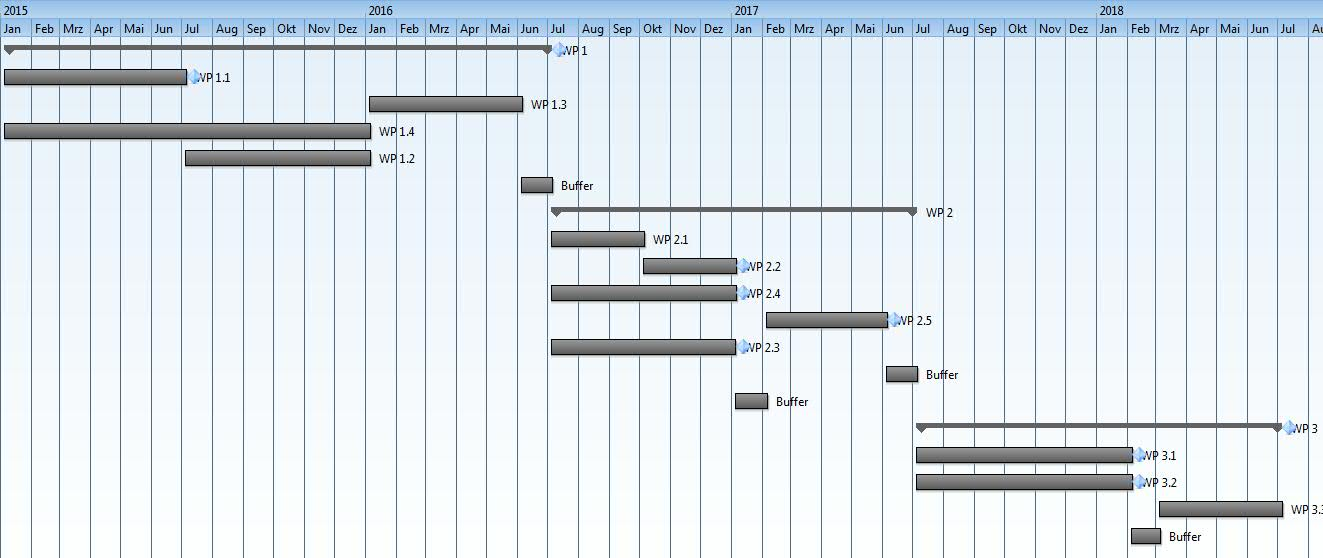
\includegraphics[width=1\textwidth]{gantt_chart}
    \caption{GANTT Chart}
\end{figure}

Each of these packages consists of another sub-packages. Since the research part of the project delivers the basis for the whole project and therefore is the most important part of the project, it has a planned duration of 1,5 years. The planned duration of the hardware and software development package is 1 year and the duration of the prototype development package 1 year. Also there is a scheduled time buffer of one month in each package, which can be used in potential problematic situations and in cases of time delays appearances. 

\subsection{Milestones}
The planned milestones of the projects are:
\begin{itemize}
\item 05.07.2015 - Confirmed uniqueness of a person’s brain wave pattern
\item 05.07.2016 - Research part completed 
\item 05.01.2017 - Hardware and Software for Microcontroller finished
\item 05.06.2017 - Hardware Part Completed 
\item 05.02.2018 - Prototype Completed 
\item 05.07.2018 - Project Completed 
\end{itemize}

\subsection{Timeplan}
The estimation of the schedule based on work packages:

\subsubsection{WP1 - Basic research}
\begin{itemize}
\item start date: 05.01.2015
\item end date:  05.07.2016
\item milestone: Research part completed
\end{itemize}


\subsubsection{WP 1.1 - Confirm uniqueness of a person’s brain wave pattern}
\begin{itemize}
\item start date: 05.01.2015
\item end date: 05.07.2015
\item milestone: Confirmed uniqueness of a person’s brain wave pattern
\end{itemize}
\subsubsection{WP 1.2 - Reliable thought identification}
\begin{itemize}
\item start date: 05.07.2015
\item end date:  05.01.2016
\end{itemize}
\subsubsection{WP 1.3 - Measuring methods of brain waves from different parts of the head}
\begin{itemize}
\item start date: 05.01.2016
\item end date: 05.07.2016
\end{itemize}
\subsubsection{WP 1.4 - Survey of state of the art for sensors and devices for brain wave measurement}
\begin{itemize}
\item start date: 05.01.2015
\item end date: 05.01.2016
\end{itemize}
\subsubsection{WP 2 - Hardware and software development}
\begin{itemize}
\item start date: 05.07.2016
\item end date:  05.07.2017
\end{itemize}

The Milestones for the work packages 2.2, 2.3 and 2.4 share the same milestone - Hardware and Software for Microcontroller finished and after this three work packages there is also planned a buffer of one month for eventual time delays.

\subsubsection{WP 2.1 - Reviewing of existing algorithms for detecting patterns in measured brain}
\begin{itemize}
\item start date: 05.07.2016
\item end date:  05.10.2016
\end{itemize}
\subsubsection{WP 2.2 - Develop new algorithms for detecting patterns in measured brain waves}
\begin{itemize}
\item start date: 05.10.2016
\item end date:  05.01.2017
\item milestone: Hardware and Software for Microcontroller finished 
\end{itemize}
\subsubsection{WP 2.3 - Define the communication protocol and interface of the Wavy}
\begin{itemize}
\item start date: 05.07.2016
\item end date:  05.07.2017
\item milestone: Hardware and Software for Microcontroller finished 
\end{itemize}
\subsubsection{WP 2.4 - Develop small sensors for brain wave measurement}
\begin{itemize}
\item start date: 05.07.2016
\item end date: 05.01.2017
\item milestone: Hardware and Software for Microcontroller finished 
\end{itemize}
\subsubsection{WP 2.5 - Develop a microcontroller for the Wavy}
\begin{itemize}
\item start date: 05.01.2017
\item end date: 05.07.2017
\item milestone: Hardware Part Completed
\end{itemize}
\subsubsection{WP 3 - Prototype development}
\begin{itemize}
\item start date: 05.07.2017
\item end date: 05.07.2018
\item milestone: Project Completed
\end{itemize}
\subsubsection{WP 3.1  - Create the Wavy prototype}
\begin{itemize}
\item start date: 05.07.2017
\item end date: 05.03.2018
\item milestone: Prototype Completed
\end{itemize}
\subsubsection{WP 3.2  - Write a software prototype}
\begin{itemize}
\item start date: 05.07.2017
\item end date: 05.03.2018
\item milestone: Prototype Completed
\end{itemize}
\subsubsection{WP 3.3  - Comparing with existing authentication methods}
\begin{itemize}
\item start date: 05.03.2018
\item end date:  05.07.2018
\end{itemize}

\subsection{Critical Areas}
The critical areas of this project are in the research part, because if the research parts doesn’t deliver the following results, the project will not fail but it won’t lead to the planned project goals. The Work package 1.1 (Confirm uniqueness of a person’s brain wave pattern) and 1.3 (Identify the methods to measure brain waves from different head parts) are the most critical parts of the project.






% --------------------------------------------------------------
\section{Human resources / team}
\label{sect:team}
\subsection{Required Persons and Roles}
\begin{itemize}
\item Project Manager
\item Neuroscience Researcher
\item Computer Science Researcher
\item Hardware Engineer
\item Software Engineer
\end{itemize}

\subsection{Project Manager}
The project managers have the responsibility of the planning, execution and closing of the project. A project manager is the person responsible for accomplishing the stated project objectives. Key project management responsibilities include creating clear and attainable project objectives, building the project requirements, and managing the constraints of the project management triangle, which are cost, time, scope and quality. He is the bridging gap between the production team and client. So he/she must have a fair knowledge of the industry they are in so that they are capable of understanding and discussing the problems with either party.

However, there are some responsibilities that are common to all project Managers, noting:
\begin{itemize}
\item Developing the project plan
\item Managing the project stakeholders
\item Managing Communication
\item Managing the project team
\item Managing the project risk
\item Managing the project schedule
\item Managing the project budget
\item Managing the project conflicts
\item Managing the project delivery
\end{itemize}
So the project manager needs the following skills:
\begin{itemize}
\item Knowledge of project management
\item General management knowledge
\item Product-specific knowledge
\item Stamina and Endurance
\item A holistic and sustainable way of thinking
\item Interpersonal and communication skills
\end{itemize}

\subsection{Neuroscience Researcher}
The main tasks of the neuroscience researcher are to prove what kind of brain waves produce recognizable patterns of the same imagination, under what circumstances brain wave scans look similar and to research if the pattern changes if the context of the person changes, like a noisy environment, strong emotions or the effect of drugs.
The neuroscience researcher works in the first time period of the project, from the 05.01.2015, where the basic research about brain waves should be done in order to achieve the expected results. There are two main scientific questions that need to be answered by the neuroscience researcher.
\begin{itemize}
\item{
First of all he should confirm or disprove the uniqueness of brain waves or define how specific brain waves of a person can be identified.
}
\item{
The second task of the researcher is to confirm the uniqueness of a persons brain waves compared with the brain waves of others. Another important factor is to confirm that the brain waves of a specific thought of a person are distinguishable from other thoughts of the same person.
}
\item{
The prototype Wavy should make it possible to indirectly watch the brains function. The activity of the neurons generates an electric field, which can be measured from  outside the skull.
}
\end{itemize}

\subsection{Hardware Engineer}                         	
The hardware engineer begins his work at the beginning of the first phase of the project and starts simultaneously with the neuroscience researcher. There already are lots of existing sensors for detecting brain waves. The main task of the hardware engineer is to look if a suitable device already exists and can be made smaller or if he has to develop a new device. He is responsible for the development of the prototype in order to show that authentication over brain waves works. Also, he needs technical knowledge about signal processing.

The goal of his work is to develop a small as possible prototype device, which makes it possible for the user to wear it in the everyday life. For that purpose, the project is in need of small as possible sensors, which will be developed by the hardware engineer during his work.

He also needs to develop a micro-controller, which manages the detection and identification of brain waves. It is working with the developed algorithm and sending it over a Bluetooth interface to a chosen device. The communication with the controller is handled with the developed software interface. Therefore, the software engineer and the hardware engineer are working closely together in the same time period.

\subsection{Computer Science Researcher}
The computer researcher identifies a persons thoughts and reviews existing algorithms for detecting patterns in measured brain waves. Since it is possible that the same thought of a person can be shown different in the brain wave, we need some patterns to confirm the measured brain waves implemented in a working algorithm with good performance. If there are not found existing algorithms the development of new ones is the goal of the computer science researcher. His tasks is also to compare the results with existing authentication methods.

The computer science researcher should have knowledge of machine learning, pattern detection, human computer interface design and signal processing. He should have worked in research projects already, where he has experienced some work with brain wave research systems.

\subsection{Software Engineer}
He is a person concerned with facets of the software development process. A software  developer may take part in design, computer programming, or software project management. They may contribute to the overview of the project on the application level rather than  component-level or individual programming tasks.  His task in the project is to work on the communication protocols and the interface of the Wavy device.

This interface should make it possible for the operation system or other developers to handle their authentication over the Wavy. He is also responsible for the prototype software, which is used by the WaveMeIn.
The software engineers working area may include:
\begin{itemize}
\item Software design
\item Implementation
\item Requirement analysis
\item {Testing, including defining/supporting acceptance testing and gathering feedback from pre-release testers}
\item {Participation in software release and post-release activities, including support for product launch evangelism}
\item {Maintenance}
\end{itemize}

\subsection{Quality Assurance Manager}
The quality assurance manager has tasks in the following areas:
\begin{itemize}
\item Controlling
\item Testing
\item Reviews
\item Developing and evaluating statistics
\end{itemize}

Controlling - the quality assurance manager controls and monitors the progress of the process, he checks if plans are realistic and if a functioning project controlling exists.

Testing - the quality assurance manager checks if the test plan is conform with the quality assurance requirements, he checks if the planed tests have been executed and he monitors the test metrics.

Reviews - the quality assurance manager has to have review-knowledge. In reviews he often plays the role of a facilitator, because he checks if the found errors have been corrected after the review process. He also checks if the planed reviews have been executed and he is responsible for the quality of the executed review.

\subsection{Work Structure}
The leader of the project is the project manager, he is responsible for the achievement of project goals, resource goals and timing goals. He is also responsible for the management and coordination of the work. The team communicates via mailing lists, scrum board and GIT. Weekly there will be SCRUM meetings and daily mini scrum meetings with duration of max. 15 minutes. Once a month meetings with all project members will be held and reviews and the work progress will be discussed.The work and the information will be stored and shared with GIT. External cooperators will not be part of the project.

% --------------------------------------------------------------
\section{Costs}
\label{sect:costs}
\subsection{Personnel}
\begin{tabular}{|l|c|c|c|c|c|c|}
\hline 
Person & \% & 1st Year & 2nd Year & 3rd Year & 4th Year & Sum \\ 
\hline 
Project Manager & 100\% & 54000,00 & 55080,00 & 56181,60 & 28652,62 & 193914,22 \\ 
\hline 
Quality Manager & 75\% & 27000,00 & 27540,00 & 28090,80 & 14326,21 & 96957,11 \\ 
\hline 
Neuroscience Researcher 1 & 100\% & 41810,00 & 42646,20 & - & - & 84856,20 \\ 
\hline 
Neuroscience Researcher 2 & 100\% & 41810,00 & 42646,20 & - & - & 84856,20 \\ 
\hline 
Computer Science R. 1 & 100\% & 41810,00 & 42646,20 & 43499,12 & 22184,55 & 150139,88 \\ 
\hline 
Computer Science R. 2 & 100\% & 41810,00 & 42646,20 & 43499,12 & 22184,55 & 150139,88 \\ 
\hline 
Hardware Engineer 1 & 100\% & 31160,00 & 31783,20 & 32418,86 & 16533,62 & 111895,67 \\ 
\hline 
Hardware Engineer 2 & 100\% & 31160,00 & 31783,20 & 32418,86 & 16533,62 & 111895,67 \\ 
\hline 
Software Engineer 1 & 100\% & 31160,00 & 31783,20 & - & - & 62943,20 \\ 
\hline 
Software Engineer 2 & 100\% & 31160,00 & 31783,20 & - & - & 62943,20 \\ 
\hline 
\textbf{SUM} & & 372880,00 & 380337,60 & 236108,38 & 120415,27 & 989325,98 \\ 
\hline 
\end{tabular} 

\subsection{Hardware}
\begin{tabular}{|l|c|c|c|c|c|}
\hline 
Item & 1st Year & 2nd Year & 3rd Year & 4th Year & Sum \\ 
\hline 
Commercial EEG Headsets & 3000,00 & - & - & - & 3000,00 \\ 
\hline 
Medical EEG Device & 60000,00 & - & - & - & 60000,00 \\ 
\hline 
Server & 4000 & - & - & - & 4000,00 \\ 
\hline 
Workstations/Notebooks & 6400,00 & - & - & - & 6400,00 \\ 
\hline 
\textbf{SUM} & 77000,00 &  &  &  & 77000,00 \\ 
\hline 
\end{tabular}

\subsection{Material}
\begin{tabular}{|l|c|c|c|c|c|}
\hline 
Item & 1st Year & 2nd Year & 3rd Year & 4th Year & Sum \\ 
\hline 
Hardware for the Prototype & 2000,00 & - & - & - & 2000,00 \\ 
\hline 
EEG Sensors & 500,00 & - & - & - & 500,00 \\ 
\hline 
\textbf{SUM} & 2500,00 &  &  &  & 2500,00 \\ 
\hline 
\end{tabular} 

\subsection{Travel Costs}
\begin{tabular}{|l|c|c|c|c|c|}
\hline 
Item & 1st Year & 2nd Year & 3rd Year & 4th Year & Sum \\ 
\hline 
Conferences & 4000,00 & - & 4000,00 & - & 8000,00 \\ 
\hline 
\textbf{SUM} & 4000,00 &  & 4000,00 &  & 8000,00 \\ 
\hline 
\end{tabular} 

\subsection{Other Costs}
\begin{tabular}{|l|c|c|c|c|c|}
\hline 
Item & 1st Year & 2nd Year & 3rd Year & 4th Year & Sum \\ 
\hline 
Team-building, Snacks, Coffee, Meetings & 7000,00 & 7000,00 & 7000,00 & 3500,00 & 24500,00 \\
\hline 
\end{tabular} 


% --------------------------------------------------------------
\section{Expected Implications and Risks}
\label{sect:implication-risk}

\subsection*{Implications and challenges}
One of the biggest challenge in the project is the basic research to detect unique brain waves. When our research has success and we are able to detect it, there are many use cases in other topics. One use case could be usage for high secure applications and systems. Where biometrical methods has some disadvantages, we have discussed above, our method can reduce this disadvantages.
Other topics could be the medicine. Current we know only a little bit about brain waves. With our research we could increase our medical understanding of brain waves.

\subsection*{Risks}

\subsubsection*{Less money}
\begin{itemize}
 \item Description: Get less money to realize the project than defined in the cost accounting.
 \item Solution: Our project is calculated tightly. So we must revalidate the hole project and create a new proposal with less features and work packages.
\end{itemize}

\subsubsection*{More money needed}
\begin{itemize}
 \item Description: The project needs more money than defined in the cost accounting.
 \item Solution: Looking for new investors to get more money. Sell know-how to other companies or research groups.
\end{itemize}

\subsubsection*{Less time for research}
\begin{itemize}
 \item Description: The brain waves research needs more time than supposed.
 \item Solution: Buy know-how from other companies and research groups. Get external experts to increase the research.
\end{itemize}

\subsubsection*{Team members leave}
\begin{itemize}
 \item Description: One or more team members leave the project.
 \item Solution: All work topics have two members. To avoid loosing knowledge, there are meetings every week to beware it. After knowledge about leaving a team member, we are looking for a new team member.
\end{itemize}

\subsubsection*{Brain waves location}
\begin{itemize}
 \item  Description: It is not possible to detect brain waves in the near of the ear.
 \item Solution: We are using sensors to detect brain waves at the forehead.
\end{itemize}

\subsubsection*{Brain waves detection}
\begin{itemize}
 \item Description: It is not possible to detect uniqueness of brain waves.
 \item Solution: It is not possible to continue, because this is the base of the project.
\end{itemize}

\subsubsection*{Misinterpretation}
\begin{itemize}
 \item Description: The team members not understand the specification correctly.
 \item Solution: Make meetings and reviews to ensure that every team member has understand it correctly.
\end{itemize}


% --------------------------------------------------------------
\section{Ethical Considerations \& Security Issues}
\label{sect:ethics-security}
\subsection{Ethical Considerations}

\subsubsection*{Electromagnetic Waves}
At the moment there is an ongoing dispute in the public over weather or not long-term exposure to electromagnetic fields can cause cancer or changes in the brain chemistry. As far as we know today weak electromagnetic fields will have no effects on the human brain, but strong fields definitively do. The Wavy device will definitely create such a weak magnetic field (like all electric devices) and due to its location at the users ear and the intention of wearing it permanently it has the potential of harming the user if electromagnetic waves really have negative effects on the human brain. 

\subsubsection*{Collecting User Data}
The Wavy device could be copied by companies trying to make a profit by constantly monitoring the emotional state of the user. The device would still function as an access device, but it could be misused for marketing purposes for example. A possible scenario could be: A company installs a wireless module into a TV set that sends a signal when an advertisement is shown. This signal activates an application in the user’s phone which in turn starts collecting emotional data via such a “bad” Wavy device from the user who is watching the advertisement. The company can then sell the gathered knowledge about the user’s response to the advertisement and his/her preferences to others such as the advertising company.

\subsection{Security Issues}
\subsubsection*{Mind Reading}
At the current state of the technology mind reading is still science fiction, but basically a device such as the Wavy could be used to read all thoughts of a user. The only real issue that is preventing this scenario at the moment is that from a given set of brain waves there is currently no way of translating this user’s thought into a visual or textual representation for someone else to read. However, this may be possible at some point in the future. A compromised Wavy device poses a serious security risk for the user.

\subsubsection*{Bluetooth}
The biggest issue in security is probably the Bluetooth connection itself. We have to rely on the Bluetooth standard to be secure, as we cannot change it and there are basically no other alternatives to Bluetooth at the moment.


% --------------------------------------------------------------
% APPENDIX
\begin{appendix}

\pagebreak

% --------------------------------------------------------------
% References
\phantomsection
\addcontentsline{toc}{section}{References}

\bibliographystyle{apalike}
\bibliography{biblography}

\pagebreak

% --------------------------------------------------------------
% Abbreviations
\section*{Abbreviations}
 \addcontentsline{toc}{section}{Abbreviations}
 
 \begin{description}
  \item[MSWP] Management von Software Projekten
  \item[WP] Work Package
 \end{description}

\end{appendix}


\end{document}
